\chapter{Methods}

\paguso{Nesta primeira revisão, eu editei algumas coisas diretamente mas deixei várias outras anotadas pra vc perceber o espírito da coisa. A ideia básica é keep it simple. Quando vc for revisar, releia as frases e veja que palavras são desnecessárias pra compreensão do texto. Se remover uma palavra ou expressão não muda o sentido do texto nem prejudica sua compreensão, não hesite: retire-as. Prefira também orações na voz ativa e na ordem direta sujeito-predicado-complemento.}

\asq{Onde falar de \kmer counting? É importante fazer essa definição para poder introduzir o \dBCM, do contrário ele vai parecer fora de lugar por não ser uma representação sucinta.}

\section{\dBG{s}}
\label{sec:dBG}

% - Detailed explanation of \dBG of a set of DNA sequences
%   - reverse complements
% - How it is going to be used
% - Operations
%   - Insert node
%   - Insert edge
%   - Query node
%   - Query edge / star 
% - Space-efficient representations - that's what we propose

The \keyterm{\dBG of order $k$} of a string \strdef{x}{n}, $G(X;k)=(V,E)$, is defined as the directed graph whose nodes $V$ represent all distinct \kmer{s} (i.e. substrings of length $k$) of \strname{X}, and such that any two nodes representing $(k-1)$-overlapping \kmer{s} are connected by an edge labeled by the last character of the second \kmer. For example if $k=3$ and $X$ contains the substring \chr{ACGT} then the consecutive triplets \chr{ACG} and \chr{CGT} will originate the edge $\chr{ACG}\stackrel{\chr{C}}{\longrightarrow}\chr{CGT}$. Hence the edges $E$ represent all distinct $(k+1)$-mers of $X$. 
% That is, given two nodes on the graph, they each represent a distinct sequence of symbols $S_1$ and $S_2$, and there is an edge between them if and only if the tail of $S_1$ is the head of $S_2$.
This definition generalizes naturally to a \emph{set of strings} \strsetname{X} by having $G$ to represent all distinct \kmer{s} of all strings in \strsetname{X}.

In genome sequencing, \dB graphs are used in the assembly process to represent the distinct \kmer{s} in a set \readset of randomly distributed fragments of the source DNA \strname{S}, called \keyterm{reads}, generated by the sequencing machines. Ideally, \strname{S} could be obtained from an Eulerian traversal of $G(\readset, k)$. Unfortunately however, due to sequencing errors and repeats, such a straightforward approach is not feasible, but the \dBG can still be used to produce a collection of partial assemblies, called \keyterm{contigs}, which can then be further combined to form the original genome \cite{Pevzner2001}. Figure~\ref{fig:dbgexample} presents an example of the \dBG in this context.

\begin{figure}[htbp]
	\begin{center}
    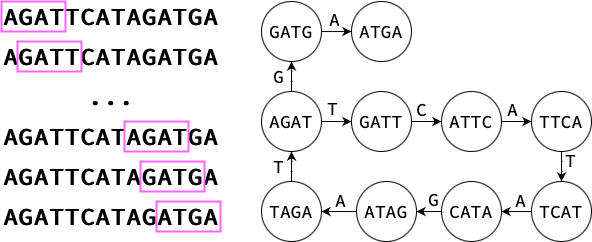
\includegraphics[width=0.8\textwidth]{figures/dbg-example}
	\end{center}
	\caption{Example of a \dBG. $k=4$}\label{fig:dbgexample}
\end{figure}

\subsection{Reverse Complements}
\label{subsec:dBG-reversecomplements}

One difficulty of using \dBG to represent DNA data is the presence of \keyterm{reverse complements}. When generating sequencing reads, the machine reads either of the two complementary strands of a fragment of the input DNA. That is, the output read may correspond to the sequence \strname{S} in the forward (5'-3') direction, or its reverse complement \strname{\overline{S}} in the backward (3'-5') direction, with
\strname{\overline{S}} being obtained from \strname{S} by swapping each base with its Watson-Crick complement
($\A \leftrightarrow \T$, $\C \leftrightarrow \G$) and then reversing the string, and vice versa. 

To deal with reverse complements, reads are processed twice\asq{can be made active? we doesn't apply as we're talking in abstract}, once in each direction. Nodes representing \kmer{s} that are reverse complements of each other can then be merged, with edges made bi-directed. Alternatively, those nodes can be kept distinct, resulting in a symmetric graph in which, as noted by Conway \& Bromage, ``a forward traversal corresponds to the backwards traversal on the reverse complement path, and vice versa.'' \cite{Conway2011}
% As in \cite{Conway2011}, this will be treated by processing
% all reads in both directions, without, however, merging nodes representing reverse complements. As noted by Conway \& Bromage: ``This
% makes the graph symmetric; a forward traversal corresponds to a backwards traversal on the reverse complement path, and vice versa.``
% \cite{Conway2011}

\subsection{Selecting the \kmer{s} for the \dBG}
\label{subsec:dBG-selectingkmers}

Another difficulty of using a \dBG to represent DNA data is dealing with sequencing errors. The set of \kmer{s} that compose the \dBG is selected from the reads in \readset. Many of those \kmer{s}, however, are not found in the original genome \strname{S}. This happens because there is an error rate associated with reading any single base from \strname{S} (0.1\%--1\% per base in Illumina \cite{Metzker2010}). As discussed by Conway \& Bromage, a single error can result in $k$ spurious \kmer{s} that appear only once in the reads. This causes the number of spurious \kmer{s} to grow proportionally to the number of bases in the reads ($\sum_{\strname{X}_i \in \readset} |\strname{X}_i|$), determined by the coverage\asq{Interesting to further discuss and define coverage? Other papers don't seem to do so}, while the number of true \kmer{s} is proportional to the size of the genome ($|\strname{S}|$) \cite{Conway2011}. Filtering these \kmer{s} is, therefore, an important aspect of constructing the \dBG.

One integral step of the filtering process is counting the \kmer{s}. A true \kmer is expected to appear in the reads a number of times equals to the coverage while, as mentioned before, many of the spurious \kmer{s} caused by sequencing errors will only appear once in all the reads.

A variety of methods for performing \kmer counting exist, each with their own set of functionalities and trade-offs. In 2014, Zhang \emph{et al.} introduced khmer \cite{Zhang2014}, a software package that performs \kmer counting through the use of a \cm sketch \asq{Cite here? Discussed below?}. This approach allows for over-counting of the \kmer{s} in exchange for better space-efficiency, allowing the counting to happen entirely in-memory. Ghosh \& Kalyanaraman later introduced \emph{FastEtch} \cite{Ghosh2019}, an assembler that used a \cm sketch to filter spurious \kmer{s} before adding them to a hashtable-based representation of a \dBG. This approach allowed them to construct the \dBG as the reads were being processed.

\subsection{\dBG representation}
\label{subsec:dBG-representation}

A \dBG can be represented either by its set of nodes (\kmer{s}) or edges ($(k+1)$-mers) equivalently, as one can be derived from the other. Therefore, a structure that can determine if a given node $x$ is a member of $G$ can represent the \dBG. Conway \& Bromage showed that the lower bound on the space required to \emph{exactly} represent these \keyterm{membership data structures} is $\Omega(n \log n)$, with $n=|V(G)|$ \cite{Conway2011}.

In order to further improve space-efficiency, new representations were created that trade deterministic exactness for a probabilistic approach. Pel \emph{et al.} showed that a probabilistic representation based on a Bloom Filter (BF) could accuratly represent a \dBG with as little as 4 bits per \kmer \cite{Pell2012}. \toconsider{They also showed that false positive rates could be as high as $15\%$ before false connectivity began to dominate the graph structure.}

However, Bowe \emph{et al.} \cite{Bowe2012} and Chikhi \& Rizk \cite{Chikhi2013} independently observed that giving up deterministic exactness isn't the only option for obtaining better space-efficiency, introducing two new representations that use $O(n)$ and $O(n \log k)$ bits, respectively, and allow for an exact traversal of the \dBG from a starting set of known member nodes. This is possible due to the fact that a \dBG is not queried for membership of random nodes, but rather potential neighbors of nodes already known to be in the graph. As such, the structures designed by the two groups do not offer a deterministically exact membership query operation, instead offering a neighborhood query operation that is exact for the members of the graph \cite{Bowe2012} \cite{Chikhi2013}. Chikhi \emph{et al.} later named this new form of representation a \keyterm{Navigational Data Structure} (NDS) and showed that the lower bound on the number of bits required to exactly represent a \dBG with an NDS is $3.24n$ \cite{Chikhi2014}.

% A \dBG can be represented either by its set of nodes (\kmers) or edges ($(k+1)$-mers) equivalently, as one can be derived from the other.
% As such, a structure that can answer queries about the presence of a given node on the graph is enough to
% represent the graph. Conway\&Bromage showed that the lower bound on the space required to
% \emph{exactly} represent a \dBG is $\Omega(n \log n)$ bits, where $n$ is the number of nodes\remove[isn't this obvious?]{,
% and $4^k > n$}\cite{Conway2011}.

% \asq{Isso precisa ser reescrito: NDSs não são necessariamente representações probabilisticas. Elas apenas substituem a consulta de presença de um nó pela consulta de vizinhança.}

% In order to further improve space-efficiency, new representations were created that trade deterministic exactness for a probabilistic approach. For instance, the so-called \keyterm{Navigational Data Structures} (NDS) have some probability of giving an erroneous answer to a membership query, 
% but can still be used to navigate the graph \cite{Chikhi2014}. This \change{definition is useful}{is} due to the fact that a \dBG is usually not queried for membership of \change{randomly selected}{random} nodes, but rather \remove{only} potential neighbors of \change{a known member node is queried}{nodes already known to be in the graph}. In the same paper where they introduce
% the idea of NDS \cite{Chikhi2014}\paguso{correct?}\asq{Esse artigo de Chikhi \emph{et al.} é a introdução e formalização do conceito de NDSs em oposição às Membership Data Structures. Em segunda leitura, porém, categorizar nossas estruturas como NDSs é incorreto porque NDSs devem dar respostas exatas para consultas de vizinhança, o que nós não garantimos.}, Chikhi \emph{et al.} also present a lower bound for the number of bits needed to represent such a structure as $3.24n$.
% In sections \ref{sec:debruijncountmin} and \ref{sec:debruijnhashtable} we will introduce two new NDS's. \asq{É necessário reiterar
% os objetivos das duas estrutas aqui, visto que isso já seria feito na introdução e é feito nas próprias sessões dedicadas a cada estrutura?}\paguso{até o momento, acho que não.}

\subsubsection{Operations}

Chikhi \emph{et al.} \cite{Chikhi2019} present the following set of operations common to many data structures for representing a \dBG \asq{Na verdade, eles falam especificamente de "set of \kmer{s}". Sendo que, no final das contas, um \dBG não deixa de ser um "set of \kmer{s}"}.

\begin{enumerate}
  \item \emph{Construction} of the data structure
  \item \emph{Insertion} of a new \kmer \asq{Tanto esse quanto o próximo eles notam se tratar de uma particularidade de um \dBG dinamico}
  \item \emph{Deletion} of an existing \kmer.
  \item \emph{Membership query}: Given a \kmer $x$, returns true iff $x \in G$
  \item \emph{Forward neighbor query}: Given a \kmer $x$ and a base $b$, returns true iff $x[1:k-1] \cdot b \in G$.
  \item \emph{Backward neighbor query}: Given a \kmer $x$ and a base $b$, return true iff $b \cdot x[0:k-2] \in G$.
\end{enumerate}

The consctruction and membership query operations are the minimum necessary, as the other operations can be derived from the two. \toconsider{An NDS, as defined in \cite{Chikhi2014}, can implement its neighborhood query by using the forward and backward neighbor queries}.

\section{An NDS based pipeline for constructing the \dBG}

\asq{Horrible section title, absolutely need to rethink this}

We propose two new probabilistic NDS-based representations for the \dBG: the \dB \cm (\dBCM), and the \dBHT. The \dBCM aims at performing online \kmer counting in a structure that can be traversed through the use of a probabilistic neighborhood query in a space-efficient manner \asq{reference the khmer or FastEtch?}. The \dBHT forgoes \kmer counting and any form of filtering in exchange for improved space-efficiency in a hashtable-based representation. Both structures aim at improving navigability on the graph by storing a set of outedges with each \kmer, allowing for \toconsider{near-}constant time neighborhood queries. These two structures can be used in tandem to leverage the benefits of each one individually: The \dBCM is constructed online as the reads are made available. Once all the reads are processed, the \dBHT is constructed by traversing the \dBCM and adding the found \kmer{s} and their outedges to the hashtable-based representation.\asq{Não faria mais sentido passar de novo pelas reads e adicionar apenas os \kmer{s} das reads que são considerados presentes? Afinal, existe uma chance de que o traversal vai passar por falsos positivos que sequer estavam nas reads. Acredito que existem duas linhas de defesa desse modelo atual: 1. como a taxa de falsos positivos vai estar mais associado a vizinhança do que ao acesso aleatório, é bem possível que falsos positivos das reads nunca sejam visitados, enquanto que \kmer{s} reais que sequer estão presentes nas reads sejam considerados como presentes por colisões, de forma que há uma chance de reduzir falsos positivos e negativos em relação a só passar pelas reads. De toda forma seria interessante uma forma de formalizar ou pelo menos testar essa hipotese}

\begin{algorithm}
  \caption{Pipeline using a \dBCM to construct a \dBHT}\label{alg:pipeline}
  \KwData{$R$, a set of sequencing reads}
  $\mathit{dBCM} \gets$ Empty \dBCM sketch\;
  \For{$\mathit{read} \in R$}{
    $\mathit{previous\_\kmer} \gets \emptyset$\;
    \For{$\mathit{kmer} \in \mathit{read}$}{
      $\mathit{dBCM}.\mathit{increment}(\kmer)$\;
      \If{$\mathit{dBCM}.\mathit{query}(\kmer).\mathit{count} \geq T$}{
        $outEdge \gets \kmer[-1]$\;
        $\mathit{dBCM}.\mathit{addOutEdge}(\mathit{previous\_\kmer}, outEdge)$\;
      }
      $\mathit{previous\_\kmer} \gets \kmer$\;
    }
    $\mathit{previous\_\kmer} \gets \emptyset$\;
    \For{$\mathit{kmer} \in \mathit{reverse\_complement(read)}$}{
      $\mathit{dBCM}.\mathit{increment}(\kmer)$\;
      \If{$\mathit{dBCM}.\mathit{query}(\kmer).\mathit{count} \geq T$}{
        $outEdge \gets \kmer[-1]$\;
        $\mathit{dBCM}.\mathit{addOutEdge}(\mathit{previous\_\kmer}, outEdge)$\;
      }
      $\mathit{previous\_\kmer} \gets \kmer$\;
    }
  }
  $\mathit{dBHT} \gets$ Empty \dBHT\;
  \For{$\kmer \in \mathit{dBCM}.\kmer{s}$}{
    $\mathit{dBHT}.\mathit{insert}(\kmer)$\;
    $\mathit{dBHT}[\kmer].\mathit{outEdges} \gets \mathit{dBCM}[\kmer].\mathit{outEdges}$\;
  }
  \Return{$\mathit{dBHT}$}
\end{algorithm}

\section{\cm}
\label{sec:countmin}

The \cm sketch \cite{Cormode2005} is a sublinear data structure for event frequency mapping.
It offers two basic operations
\begin{compactenum}
\item $update(e, f)$, and
\item $query(e)$,
\end{compactenum}
respectively for informing the occurrence of an event $e$ with frequency $f$, and for obtaining an estimate of the accumulated frequency of event $e$ up to that point.

The sketch is composed of a $D\times W$ matrix of counters $C$, and a set of $D$ pairwise-independent hash functions $h_0\ldots h_{D-1}$, such that each $h_i$ maps an event to one of the $W$ cells in row $i$.


Updating an event is done by passing it through the hash functions for each row, and then incrementing the counters in
the mapped positions $h_i(e)$ accordingly. 
We consider the simpler case where we only report individual event occurrences, so that counters are always incremented by one.

Querying the structure consists in retrieving the value of the counters associated with the key event in each row,  and then returning
the minimum value among them, that is $\min\{C[i][h_i(e)]]; i=0\ldots D-1$\}.


Figure \ref{fig:countminexample} presents a visualization of the \cm sketch.

\begin{figure}[htbp]
	\begin{center}
    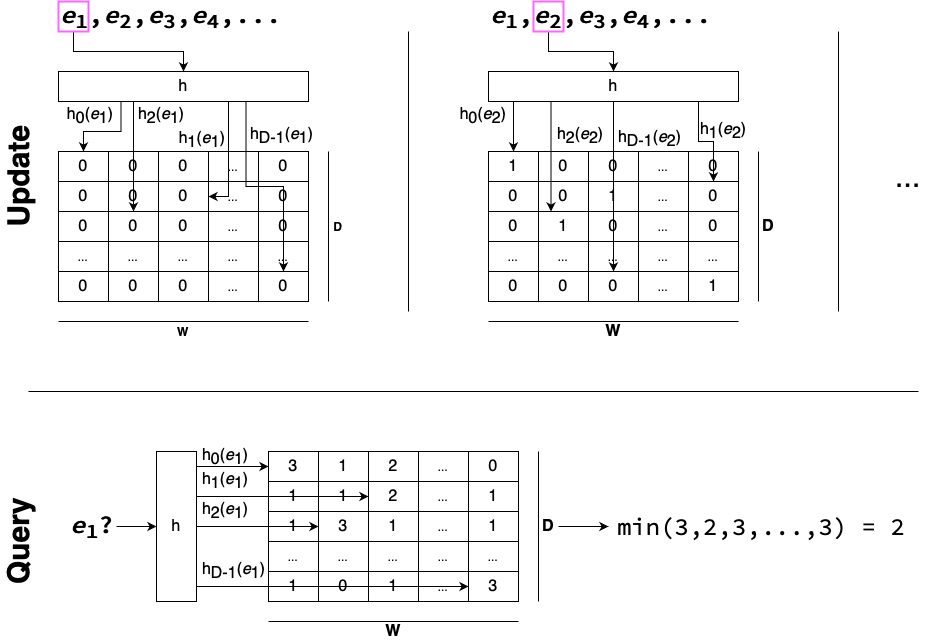
\includegraphics[width=0.9\textwidth]{figures/cm-example}
	\end{center}
	\caption{Example of a \cm sketch}\label{fig:countminexample}
\paguso{A ideia da figura está boa, mas precisa aumentar a fonte pra não ficar ilegível. Se não couber, simplifica a parte do incremento. Muda o label de Increment para Update.}
\end{figure}

It is important to notice that the \cm might overestimate the frequency of an event due to hash collisions, since more than one event might be mapped to the same cell of the matrix. However, the pairwise independence requirement ensures that, for any row $i$ and any two distinct events $e\neq e'$,
\begin{equation*}
\prob[h_i(e)=h_i(e')] = 1/W,
\end{equation*}
with this probability being computed over all possible choices of the hash function.
Hence, by setting $W$ appropriately, we can control the expected number of collisions per row, and likewise, by choosing a sufficiently large $D$, we can control for the probability of having at least one row without collisions for a given event. In general, for two given parameters $\epsilon, \delta \in (0,1)$, by setting 
$W=2/\epsilon$ and $D=\log1/\delta$, we have
\begin{equation*}
\prob[C.query(e) - f(e) > \epsilon F] < \delta,
\end{equation*}
where $f(e)$ represents the true frequency of $e$, and $F=\sum_{e_i}f(e_i)$ is the true total event count. Put another way, we can have the estimate error relative to the total event count to be `small' (no more than $\epsilon$) with `good' (at least $1-\delta$) probability.

\subsection{\cm as an intermediate representation for \dBG{s}}

A \cm sketch can implement the membership query operation by querying the count for a given \kmer and comparing it to a presence threshold:
if the count surpasses this threshold, the \kmer is considered to be present in the \dBG, and if the count is inferior to the threshold the
\kmer is considered absent from the graph.\paguso{Qual é a rationale pra isso? Precisa explicar. Aqui deve ser introduzida a questão da cobertura.}\asq{Acredito que isso agora fica claro devido a adição da seção~\ref{subsec:dBG-selectingkmers}}

\section{The \dB\cm sketch}
\label{sec:debruijncountmin}

% - Representation (what goes in each cell)
% - Operations:
%   - addOutEdge
%   - query 
% - Analysis space/time (may be done within previous sections)

Because we expect each \kmer from the sequence to appear in the reads a number of times equals to the coverage, while spurious \kmer{s} will appear a low number of times \cite{Conway2011} \cite{Ghosh2019}, a structure used to count \kmer{s} (that implements the $\mathit{count}(x)$) can implement the membership query operation as $\mathit{memb}(x)=\mathit{count}(x) \geq t$. In this way, a \cm sketch can \toconsider{probabilistically} represent a \dBG with some false positive and false negative rates associated with the membership query operation. These rates can be controlled by $t$.\asq{Aqui talvez valha a pena falar que existem duas abordagens para tentar controlar as taxas de falsos positivos e negativos: 1. O valor de $t$ pode ser estabelecido, e, então, os valores de $W$ e $D$ são calculados de forma a minimizar a chance de um erro $\epsilon > t$; 2. Os valores $W$ e $D$ podem ser fixados, e, então, $t$ é decidido baseado nas estimativas esperadas para um \kmer espúrio \emph{vs.} um \kmer real.}

Selecting the appropriate value for $t$ is not a trivial task, however, and is a trade-off between the false positive and false negative rates. Due to the fact that reads are generated randomly from the original genome, and that a number of real \kmer{s} will be replaced by spurious \kmer{s} because of sequencing errors, an universally optimal threshold \toconsider{that perfectly decides if a \kmer is spurious or not} does not exist. Higher values of $t$ are more likely to cut out spurious \kmer{s}, reducing false positive rates, but they also increase the chances of a real \kmer being missed, increasing false negative rates. Lower values of $t$ result in the opposite effect happening.

In order to leverage the benefits of an NDS in reducing the impact of the false positive rate of the membership operation, we introduce a modified version of the \cm sketch, called \keyterm{\dB\cm} (\dBCM) allowing for querying not only for \kmer counts, but also for the outedges from the corresponding nodes in the \dBG.


To store the additional information, we expand the \cm sketch such that each cell $C[i,j]$ in the matrix stores not only the counter $C[i,j].C$, but also a set of out-edges $C[i,j].E$. The structure then provides an operation to \emph{update} the counters $C[i,h_i(x)].C$ associated with a given \kmer $x$ by one, and an operation to \emph{add an out-edge} to the sets $C[i,h_i(x)].E$. The update operation is the same as in a regular \cm, and the procedure for adding an edge can be seen in Algorithm~\ref{alg:addOutEdge}.


\begin{algorithm}[htbp]
    \caption{ADD-OUTEDGE($CM, x, a$)}\label{alg:addOutEdge}
    \Input{$\mathit{CM}$, the \dBCM; $x$, the \kmer; $a \in \{\A, \C, \G, \T\}$, the outedge label}
    \For{$i \gets 0, \ldots, D-1$}{
      $\mathit{CM}[i,h_i(x)].E \gets \mathit{CM}[i,h_i(x)].E \cup \{a\}$\;
    }
\end{algorithm}

Furthermore, the \dBCM must accommodate this new information in its query operation. The sketch now returns not only the minimum value of the counters, but also the intersection of the sets of out-edges, as shown in in Algorithm~\ref{alg:query}.

\begin{algorithm}
	\caption{QUERY($CM$, $x$)}\label{alg:query}
  \Input{$\mathit{CM}$, the \dBCM; $x$, the \kmer}
  \Output{The estimated count $C$ and outedge set $E$}
	$C \gets \mathit{inf}$\;
	$E \gets \{\A, \C, \G, \T\}$\;
	\For{$i = 1, \ldots, D$}{
		$C \gets \min(C, \mathit{CM}[i,h_i(x)].C)$\;
		$E \gets E \cap \mathit{CM}[i,h_i(x)].E$\;
	}
	\Return{$(C, E)$}
\end{algorithm}

From a practical perspective, due to a node having at most four outedges corresponding to the bases $\{\A, \C, \G, \T\}$, the set storing them can be represented with four bits indicating whether each of them is present. An edge is added by setting the corresponding bit, and the intersection is obtained by performing the bitwise AND operation. Moreover the set of outedges and the counter are packed together in a single 16-bit integer. This layout can be visualized in Figure~\ref{fig:dbcm-bit_use}. When using a $k$ such that $4^k > |S|$, the each \kmer in $S$ is expected to appear only once. As such, it is expected to appear a number of times equals to the coverage $C$ in the reads. Considering that $C$ is not a very high value (commonly below $200$ \asq{Citation Needed?}), each counter can be represented by a 12-bit integer, accounting for the expected count for all real \kmer{s}, as well as any possible collisions.

\begin{figure}[htbp]
  \centering
  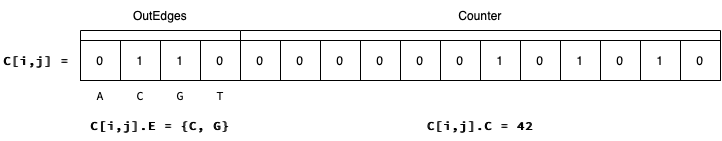
\includegraphics[width=0.9\textwidth]{figures/dbcm-bit_use}
  \caption{A cell from the \dBCM}\label{fig:dbcm-bit_use}
\end{figure}

\subsection{Using the \dBCM as a navigational structure}

\asq{Vale a pena explicitar como cada uma das operações do \dBG é implementada no \dBCM a partir das operações do \cm?

Construction $\Rightarrow$ Inicialização da matriz $W \times D$ e processamento das reads\\
Insertion $\Rightarrow$ Incremento do contador do \kmer\\
Deletion NÃO IMPLEMENTADA\\
Membership query $\Rightarrow$ QUERY($\mathit{CM}$, $x$).C $\geq t$\\
Forward neighbor query $\Rightarrow$ QUERY($\mathit{CM}$, $x$).E $\subseteq \{a\}$\\
Backward neighbor query NÃO IMPLEMENTADA}

This structure can be navigated from an initial set of \kmer{s} by querying for their out-edges and then querying each of their neighbors, repeating this for each neighbor found to be in the graph. This procedure can be observed in Algorithm~\ref{alg:traversal}.

\begin{algorithm}
	\caption{TRAVERSE($CM$, $\strsetname{S}$, $t$)}\label{alg:traversal}
  \Input{$\mathit{CM}$, the \dBCM; $\strsetname{S}$, the set of starting \kmer{s}; $t$, the threshold of presence}
  \Output{\asq{Not sure what to put here. O conjunto de \kmer{s} visitados? O conjunto de \kmer{s} consultados junto com o resultado da consulta?}}
  $F \gets$ empty Queue\;
  \For{$s \in \strsetname{S}$}{
    enqueue($F$, $s$)\;
  }
  $V \gets \{\}$\;
  \While{$F$ is not empty} {
    $u \gets$ dequeue($F$)\;
    $V \gets V \cup \{u\}$\;
    $C, E \gets QUERY(\mathit{CM}, u)$\;
    \If{$C \geq t$}{
      \For{$a \in E$}{
        $v \gets$ extend($u$, $a$)\;
        \If{$v \notin V$}{
          enqueue($F$, $v$)\;
        }
      }
    }
  }
	\Return{}
\end{algorithm}

\subsubsection{Selecting the starting set $\strsetname{S}$ of \kmer{s} for traversal}

Ideally, only the first \kmer from the original sequence is \asq{would be?} needed to perform the traversal of the graph. It isn't possible to determine, however, where in the original sequence a read was taken from\asq{Tem os casos em que dá pra colocar um pre-fixo e um pós-fixo na sequência?}. One option is to use all the \kmer{s} from the reads that are found to be in the graph. This set can be constructed during construction of the \dBCM by evaluating if a newly incremented \kmer{'s} count surpasses the established threshold. This would create an unnecessarily large set, however: \toconsider{Suppose $x_1$ and $x_2$ are  real \kmer{s} found in a same read and $x_1$ appears before $x_2$. We expect $x_2$ to be reachable in the \dBG from $x_1$, and thus it does not add any aditional information by being in $\strsetname{S}$.} We can, therefore, reduce the size of $\strsetname{S}$ by only considering the \kmer{s} that are at the start of their reads. To avoid the case where the first \kmer in each read is erroneous, we can take the first $n$ \kmer{s} from each read. \toconsider{In practice, however, this proved to be unnecessary, with $n=1$ still allowing for the complete traversal of the graph.}

\section{A space-efficiente Hashtable representation for \dBG{s}}
\label{sec:debruijnhashtable}
% - Structure
%   - fingerprint
%   - Outedges
% - Hash function 
% - Collision resolution
% - Operations 
%   - Add node/edge
%   - Query node/edge/star 
% - Analysis 
\paguso{repetindo, é necessário ter discutindo *antes* como essa coisa da hashtable vai colar com o \dBCM, senão isso parece que caiu do céu como uma coisa separada}

We also propose a new hashtable-based representation for the \dBG that is made more efficient by not storing the \kmer. Instead,
a fingerprint generated from the \kmer is stored, along with the set of out edges as described in Section \ref{sec:debruijncountmin}.
When a \kmer is inserted into the hashtable, or queried from it, a hash value and a fingerprint are calculated in parallel.
In case of an insertion, the fingerprint is written at the desired position and, on a query, the fingerprints are compared. Collisions
are resolved by linear probing, such that if a key tries to insert in a position that is already occupied by a fingerprint that doesn't 
match its own, the \kmer is inserted in the next free position, unless its fingerprint is found before a free position is. During the
query this process is repeated until the desired fingerprint is found, or a free position is reached (in which case the \kmer is
considered to be absent from the structure).

This operation allows for the insertion of a node by adding the \kmer to the hashtable, as presented in Algorithm \ref{alg:ht-insert},
and the insertion of an edge by updating the edge set associated with the given \kmer, presented in Algorithm \ref{alg:ht-addedge}.
When queried, the structure returns the edge set associated with the given \kmer, provided the \kmer has been added to the structure.
This operation is defined in Algorithm \ref{alg:ht-query}.

\begin{algorithm}
  \caption{Insert \kmer in \dBHT}\label{alg:ht-insert}
  \KwData{$\kmer$}
  $\mathit{hash} \gets \mathit{fibonacci\_hash}(\kmer)$\;
  $\mathit{pos} \gets \mathit{hash}$\;
  \While{$!\mathit{HT}[\mathit{pos}].empty \wedge \mathit{pos} \neq \mathit{hash} - 1$}{
    \eIf{$\mathit{HT}[\mathit{pos}].\mathit{fingerprint} \neq \mathit{fingerprint}(\kmer)$}{
      $\mathit{pos} \gets (\mathit{pos} + 1) mod |HT|$\;
    }{
      \Return{}
    }
  }
  \If{$\mathit{HT}[\mathit{pos}].empty$}{
    $\mathit{HT}[\mathit{pos}].\mathit{kmer} \gets \kmer$\;
    $\mathit{HT}[\mathit{pos}].\mathit{outEdges} \gets \emptyset$\;
    $\mathit{HT}[\mathit{pos}].\mathit{fingerprint} \gets \mathit{fingerprint}(\kmer)$\;
  }
\end{algorithm}

\begin{algorithm}
  \caption{Add out-edge to \kmer in \dBHT}\label{alg:ht-addedge}
  \KwData{$\kmer$, $\mathit{outEdge} \in \{\A, \C, \G, \T\}$}
  $\mathit{hash} \gets \mathit{fibonacci_hash}(\kmer)$\;
  $\mathit{pos} \gets \mathit{hash}$\;
  \While{$!\mathit{HT}[\mathit{pos}].empty \wedge \mathit{HT}[\mathit{pos}].\mathit{fingerprint} \neq \mathit{fingerprint}(\kmer) \wedge \mathit{pos} \neq \mathit{hash} - 1$}{
    $\mathit{pos} \gets (\mathit{pos} + 1) mod |HT|$\;
  }
  \If{$!\mathit{HT}[\mathit{pos}].empty \wedge \mathit{HT}[\mathit{pos}].\mathit{fingerprint} = \mathit{fingerprint}(\kmer)$}{
    $\mathit{HT}[\mathit{pos}].\mathit{outEdges}.\mathit{add}(\mathit{outEdge})$
  }
\end{algorithm}

\begin{algorithm}
  \caption{Query \kmer in \dBHT}\label{alg:ht-query}
  \KwData{$\kmer$, $\mathit{outEdge} \in \{\A, \C, \G, \T\}$}
  $\mathit{hash} \gets \mathit{fibonacci_hash}(\kmer)$\;
  $\mathit{pos} \gets \mathit{hash}$\;
  \While{$!\mathit{HT}[\mathit{pos}].empty \wedge \mathit{HT}[\mathit{pos}].\mathit{fingerprint} \neq \mathit{fingerprint}(\kmer) \wedge \mathit{pos} \neq \mathit{hash} - 1$}{
    $\mathit{pos} \gets (\mathit{pos} + 1) mod |HT|$\;
  }
  \If{$!\mathit{HT}[\mathit{pos}].empty \wedge \mathit{HT}[\mathit{pos}].\mathit{fingerprint} = \mathit{fingerprint}(\kmer)$}{
    \Return{$\mathit{HT}[\mathit{pos}].outEdges$}
  }
\end{algorithm}

\subsection{Modular Fibonacci Hashing}

The \kmer is hashed using the Fibonacci hashing algorithm, which is an algorithm that leverages a property of the golden ratio
to produce a very uniform hash distribution while also having subsequent keys be hashed to values distant from each other. The
function was modified, however, to use modular arithmetic instead of a bitwise shift operation to map the result to the intended
range. This was done in order to allow for more freedom in the choice of the desired range and, therefore, the size of the
hashtable. The algorithm for this modified version of the Fibonacci hashing function can be seen in Algorithm \ref{alg:fibonacci-hash}.

\begin{algorithm}
  \caption{Fibonacci Hash Function}\label{alg:fibonacci-hash}
  \KwData{$\mathit{key}$; $\mathit{range\_max}$}
  \Return{$(11400714819323198485 \times \mathit{key}) \mod \mathit{range\_max}$}
\end{algorithm}

\subsection{Fingerprint}

When performing the Fibonacci hashing, the most significant bits of the result of the multiplication are discarded by the modulo.
Those bits are also distributed uniformly over the possible keys, such that they can be used as a fingerprint for the \kmer.
As such, the fingerprint function can be defined as in Algorithm \ref{alg:fingerprint}. \asq{Existe uma forma melhor de formalmente
escrever que os $n$ bits mais significativos são escolhidos?}

\begin{algorithm}
  \caption{Fingerprint Function}\label{alg:fingerprint}
  \KwData{$\mathit{key}$}
  \Return{$(11400714819323198485 \times \mathit{key}) >> 61$}
\end{algorithm}

\section{Experiments}

\subsection{Metrics}

\asq{Is accuracy the best term here? Why not precision, for example? Is there a more suitable term?}

\subsubsection{Representation Accuracy of a \dBCM}

The \dBCM aims at two things: (1) to count the \kmer{s} from the reads, and (2) to represent a navigatable \dBG. Due to its probabilistic nature, however, it will not achieve deterministic exactness in either of those aims. It becomes interesting, therefore, to evaluate how accurate it is at them. To do so, we compare its estimated count for each of the \kmer{s} in the reads to the \kmer{s} actual count. We also test the false positive and false negative rates of the sketch before traversal.

\paragraph{Count Accuracy} To evaluate count accuracy, we compare the estimated count for each \kmer in the reads with its actual count. We compare the count distributions, as well as evaluate \asq{repeat evaluate?} the average error and the standard deviation of the errors.

\paragraph{False Positives} False positives occur when a \kmer that is not found in the original DNA sequence $\strname{S}$ is considered to be present in the \dBG. In a \dBCM this happens when the estimated count for that \kmer is above the determined presence threshold.

\paragraph{False Negatives}

\subsubsection{Graph Traversal}

As noted by Bowe \emph{et al.} \cite{Bowe2012} and Chikhi \& Rizk \cite{Chikhi2013}, the \dBG isn't queried for random nodes, but rather for the neighbors of a known member node. \asq{repeat this or mention the ``discussion'' in Section \ref{subsec:dBG-representation}} It becomes interesting, therefore, to evaluate it in these circumstances. To do so, we perform a traversal of the graph starting from a subset of the \kmer{s} taken from the reads. We store the \kmer{s} that are queried for, as well as the query result. We can, then, count the number of distinct \kmer{s} queried, as well as the number of those that were found to be in the graph. We further use that to determine the false positive and false negative rates. \toconsider{It is importante to make the distinction between these rates when performing the traversal of the graph \emph{versus} as they were introduces in the previous section: the false positive rate is potentially lower, while the false negative rate is potentially higher. This happens because \kmer{s} that would be considered present in the graph might have all of its backwards extensions be considered absent, in which case it will never be queried for.}

\paragraph{False Positives}

\paragraph{False Negatives}

\subsection{\emph{E.~Coli}}

\subsubsection{Synthetic Reads without Errors and Reverse Complements}

\subsubsection{Synthetic Reads without Errors and with Reverse Complements}

\subsubsection{Synthetic Reads with Errors}

Through the experiments described further in this section, we evaluate different metrics for the \dBCM and the \dBHT. This is due to
the fact that both these structures have different goals and are used in different contexts.

As both of these structures are probabilistic in nature, however, there are certain metrics that are used in the evaluation of both.
One such metric is the \emph{false positive rate}. We define this rate based on the \kmer{s} that are visited during a 
traversal of the graph. Let $S$ be a genetic sequence that contains the set of \kmer{s} $K$, and let $G$ be the graph, represented
either by a \dBCM or a \dBHT, constructed from the sequencing reads of $S$. Further, let $Q$ be the set of \kmer{s} that were queried
from $G$ during its traversal, and $P=\{k | k \in Q \wedge k \in graph\}$ be the set of queried \kmer{s} that were in $G$. As such, we can
define the set of false positives as $F_P=P \setminus K$ (i.e. the set of \kmer{s} that were queried and found to be in $G$ but are not
actually in the original sequence $S$). Finally, the false positive rate is defined as $\mathit{fp}=\frac{|F_P|}{|Q|}$ (i.e. the
proportion of \kmer{s} found during traversal of $G$ that are not found in $K$).

\asq{Realmente vale a pena tentar fazer isso ainda? Estamos na reta final do projeto já, e isso iria requerer a definição do que é uma
mudança significativa nos resultados que justifique a mudança na estrutura}

As we posit that adding the out-edge information to the structures will improve its navigability by reducing the chances of generating
false branches on the graph, we also look at the number of out-edges found for each \kmer in the graph. We can look at the distribution
of these results as a way to evaluate the possible impact of this aditional information: the more \kmer{s} that have fewer out-edges,
the fewer forks there are, and the less likely that a false branch will be generated. \asq{Provavelmente é válido gerar uma formalização
desse conceito de distribuição da contagem de out-edges por \kmer}. Beyond that, we also perform the traversal of the graph with and
without using the out-edge information, such that we can compare the results and measure the impact in this way.

\subsubsection{\dBCM}

The \dBCM was developed to be used directly with the sequencing reads without any pre-processing. It's goal is to build a reliable
navigatable version of the \dBG as the reads are made available. In this context, not only do we expect a certain amount of false
positives will appear, but as we must probabilistically filter the set of \kmer{s} from the reads to remove all the spurious ones, we
also expect the occurence of \emph{false negatives}, which are defined as \kmer{s} from the original sequence $S$ that are not present
in the graph $G$. I.e.: $F_N=K \setminus P$. As such, the \emph{false negative rate} can be defined as the ratio of false negatives
to the total number of \kmer{s} in the original sequence $S$, or $\mathit{fn}=\frac{|F_N|}{|K|}$.

\subsubsection{\dBHT}

\subsection{\emph{E.~Coli}}

The \emph{E.~Coli} genome is an established benchmark for new assemblers to compare against. We used the reference chromossomal dna
genome made available by Ensembl Genomes for the strain k 12, substrain mg1655 of this species\cite{ecoligenome}.

% We used the reference genome for the \emph{E.~Coli} bacterium available in \url{http://ftp.ensemblgenomes.org/pub/bacteria/release-52/fasta/bacteria_0_collection/escherichia_coli_str_k_12_substr_mg1655_gca_000005845/dna/}

Three different experiments were performed. In the first we generated simulated perfect reads from the genome by taking substrings of 
the original sequence at random. We then used the \emph{ART Illumina} toolkit \cite{Huang2011} to simulate realistic reads from this
genome, including read errors and reverse complements. \toconsider{Finally, a dataset of real-world reads was downloaded from SRA \cite{Leinonen2011}
and used.}
\asq{Eu mencionei esse último teste na esperança que dê tempo de realiza-lo ainda.}

\subsubsection{Synthetic reads without errors}

Given the reference genome $S$, the length of each read, $L$, and the desired coverage $C$, the synthetic reads were generated by picking
$\frac{|S| \times C}{L}$ substrings of $S$ at random. This is presented in algorithmic form in Algorithm \ref{alg:generate-reads}.

\begin{algorithm}
  \caption{Generate Reads}\label{alg:generate-reads}
  \KwData{$S$, the reference genome, $L$ the read length, $C$ the coverage}
  $\mathit{\#reads} \gets \frac{|S| \times C}{L}$\;
  $reads \gets \emptyset$\;
  \For{$i \gets 1, \ldots, \mathit{\#reads}$}{
    $j \gets \mathit{random}(0, |S| - L)$\;
    $\mathit{reads.add}(S[j: j+L])$\;
  }
  \Return{$reads$}
\end{algorithm}

\subsubsection{Synthetic reads with errors}

In order to simulate the reads as they would be produced by the sequencing process, we used the ART Illumina toolkit to generate
synthetic reads from the \emph{E.~Coli} genome. The reads were generated using the following parameters:

\begin{enumerate}
\item \textbf{Sequencing System}: Illumina MiSeq v3
\item \textbf{Read length}: \textit{250bp}
\item \textbf{Coverage}: \textit{80x}
\end{enumerate}